\section{Problem Statement}\label{sec:problem_statement} 

\gls{eeg} is one of the most widely adopted technologies for \gls{mi}--based \glspl{bci} due to its non-invasive nature, low cost, portability, and high temporal resolution~\cite{singh2021comprehensive}. However, \gls{eeg} signals are intrinsically affected by structural and physiological limitations that hinder their effective exploitation in real-world applications. In particular, low spatial resolution, high susceptibility to noise and physiological artifacts, and volume conduction effects complicate the localization and physiological interpretation of cortical sources~\cite{wang2019eeg}. Furthermore, the nonlinear and nonstationary nature of \gls{eeg} signals poses additional challenges for robust modeling and analysis, limiting the reliability and interpretability of conventional \gls{eeg}-based \gls{bci} systems, especially in clinical and rehabilitation contexts where stable and explainable neural decoding is required~\cite{bouazizi2024interpretability}.

Beyond signal-level limitations, \gls{eeg}-based \glspl{bci} are strongly affected by pronounced inter-subject and intra-subject variability, leading to heterogeneous neural activation patterns across users and recording sessions~\cite{kim2023bridging,maswanganyi2022statistical}. This variability hampers generalization, promotes subject-dependent models, and contributes to the well-known BCI illiteracy phenomenon, where a significant proportion of users fail to achieve reliable control~\cite{saha2020intra,horowitz2021external}. Although deep learning approaches have improved decoding performance, many existing models rely on rigid or opaque representations that limit neurophysiological interpretability and fail to capture dynamic and nonlinear dependencies between \gls{eeg} channels~\cite{shoka2019literature,zhang2015bayesian}. These limitations highlight the need for connectivity-aware and interpretable learning frameworks capable of modeling complex brain interactions while improving robustness and generalization in \gls{mi}-based \gls{bci} systems~\cite{rolls2022effective}.

In this context, the following subsections provide a detailed analysis of the main challenges addressed in this thesis within the scope of EEG-based BCI systems, focusing on noisy data and low spatial resolution (Subsection~\ref{sec:Noisy}), nonlinear and nonstationary EEG channel dependencies (Subsection~\ref{sec:nonlinear}), and high inter- and intra-subject variability (Subsection~\ref{sec:variability}).

\subsection{Noisy data and low spatial resolution}\label{sec:Noisy}


One of the most critical limitations of \gls{eeg}-based \gls{bci} systems is their inherently low spatial resolution, which stems from the physical process by which neural electrical activity propagates from cortical sources to scalp electrodes. Due to volume conduction effects, \gls{eeg} signals traverse multiple tissue layers with heterogeneous conductivities, such as the cerebrospinal fluid, skull, and scalp, before being recorded. This phenomenon leads to spatial blurring and mixing of neural sources across electrodes, making it difficult to accurately localize task-related cortical activations~\cite{wang2019eeg}, as schematically illustrated in Figure~\ref{fig:problem1}. As a consequence, spatial specificity is significantly reduced compared to imaging modalities such as \gls{fmri} or \gls{meg}, limiting the effectiveness of \gls{eeg}-based \glspl{bci} in applications that require precise discrimination of motor and sensorimotor regions and impairing the interpretability of learned representations~\cite{electronics12122743,pan2025enhancing}. This challenge is particularly critical in \gls{mi}-based \gls{bci} paradigms and neurodevelopmental conditions such as \gls{adhd}, where motor-related cortical activations tend to be weaker, more diffuse, and highly variable, further exacerbating source localization uncertainty and reducing the reliability of neurophysiological interpretation~\cite{alnuaimi2022adhdmi}.

\begin{figure}[H]
    \centering
    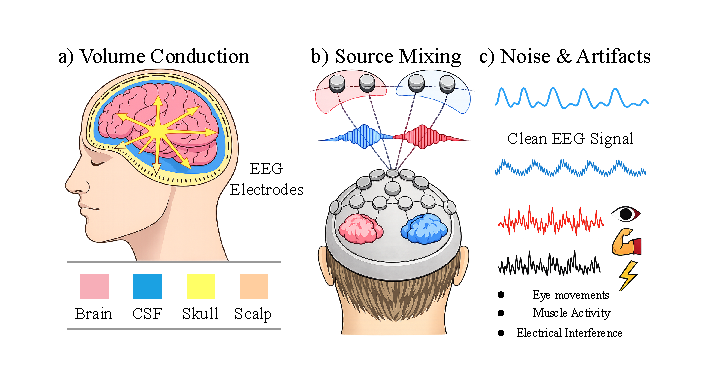
\includegraphics[width=\linewidth]{Figures/Problem 1.pdf}
    \caption{Major factors limiting \gls{eeg} spatial specificity and signal quality: (a) volume conduction through CSF, skull, and scalp causes spatial smearing; (b) source mixing leads each electrode to record a linear combination of multiple cortical sources; and (c) physiological and environmental artifacts (e.g., eye movements, muscle activity, and electrical interference) degrade the signal-to-noise ratio.}
    \label{fig:problem1}
\end{figure}

In parallel with limited spatial resolution, \gls{eeg} recordings are highly vulnerable to noise and artifacts arising from both physiological and non-physiological sources, including ocular movements, muscle activity, head motion, and environmental interference~\cite{de2018agenda}. These contaminations often overlap spectrally with task-relevant rhythms, such as the $\mu$ and $\beta$ bands, which are fundamental for \gls{mi} decoding~\cite{pfurtscheller1999event}. As a result, the signal-to-noise ratio is substantially degraded, increasing intra- and inter-trial variability and reducing the robustness of conventional feature extraction and classification pipelines~\cite{bouazizi2024interpretability}. Although classical preprocessing techniques and spatial filtering methods can partially mitigate these effects, they remain sensitive to residual noise and spatial distortions, ultimately constraining the generalization capability and reliability of \gls{eeg}-based \gls{bci} systems in real-world and clinical settings~\cite{akuthota2023complete,pan2025enhancing}, particularly in \gls{mi}-based applications and populations with \gls{adhd}, where attentional fluctuations, involuntary movements, and reduced task compliance further degrade signal quality and stability~\cite{lenartowicz2018adhd}. These limitations motivate the need for representations that go beyond sensor-level activity and explicitly model inter-channel relationships, including their nonlinear and time-varying dynamics, to improve robustness and interpretability under noisy and low-resolution \gls{eeg} conditions.

\subsection{Nonlinear and Nonstationary \gls{eeg}Channel dependencies}\label{sec:nonlinear}

\gls{eeg} signals exhibit pronounced nonlinear and nonstationary behavior, reflecting the intrinsic dynamics of underlying neural processes and their continuous adaptation to cognitive states, stimuli, and task demands~\cite{breakspear2017dynamic}. In \gls{mi} paradigms, the statistical properties of \gls{eeg} signals vary over time due to changes in attention, mental strategy, and neural engagement, which violates the assumptions of stationarity commonly adopted by classical signal processing and machine learning methods~\cite{shoka2019literature}. These effects are further exacerbated in practical \gls{eeg}-based \glspl{bci}, where variability across trials, sessions, and subjects introduces additional sources of nonstationarity that challenge reliable decoding. Moreover, neural interactions across cortical regions are inherently nonlinear, as they arise from complex synaptic mechanisms, recurrent feedback loops, and cross-frequency interactions. Such nonlinear dynamics are particularly relevant in neurodevelopmental conditions such as \gls{adhd}. {Clinically, ADHD is characterized by persistent patterns of inattention and/or hyperactivity--impulsivity that interfere with functioning or development~\cite{APA2022DSM5TR}.} In this context, altered
attentional control and fluctuating cognitive states have been associated with abnormal neural coupling and increased temporal variability. These characteristics limit the effectiveness of linear connectivity measures and static feature representations, which are unable to fully capture the evolving and nonlinear dependencies that govern inter-channel \gls{eeg} dynamics~\cite{rolls2022effective}. These nonlinear, nonstationary, and time-evolving inter-channel interactions are schematically illustrated in Figure~\ref{fig:problem2}.

Beyond nonstationarity, \gls{eeg} channels interact through time-delayed and directed relationships that reflect causal information flow within brain networks~\cite{rolls2022effective}. In \gls{eeg}-based \glspl{bci}, particularly those relying on \gls{mi} decoding, capturing such directed interactions is essential for distinguishing task-relevant sensorimotor activations from background or confounding activity. Conventional correlation-based or symmetric connectivity measures fail to adequately characterize these interactions, as they cannot distinguish between driving and responding channels nor capture nonlinear dependencies~\cite{zhang2015bayesian}. This limitation is especially critical in high-variability scenarios, including subject-independent \gls{bci} operation and neurodevelopmental studies involving \gls{adhd}, where spurious or volume-conduction-driven correlations may obscure meaningful patterns of effective connectivity. Information-theoretic approaches, such as \gls{te}, have been proposed to quantify directed and nonlinear interactions between time series~\cite{schreiber2000measuring,staniek2008symbolic}. However, their practical application to \gls{eeg} signals is hindered by high sensitivity to noise, high data dimensionality, and the need for explicit probability density estimation, which limits their effectiveness in real-world \gls{bci} scenarios characterized by nonstationary and noisy \gls{eeg} recordings~\cite{pereda2005nonlinear}.These nonlinear, nonstationary, and directed inter-channel dependencies are not only task- and state-dependent, but also vary substantially across individuals and recording sessions, naturally giving rise to pronounced inter- and intra-subject variability in \gls{eeg}-based \glspl{bci}.

\begin{figure}[h]
    \centering
    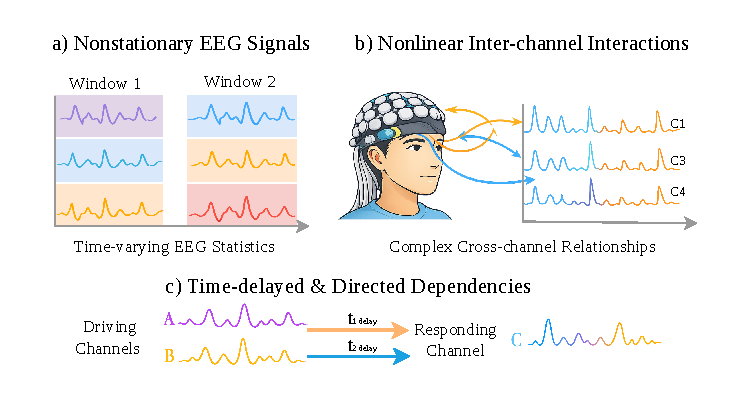
\includegraphics[width=\linewidth]{Figures/Problem 2.pdf}
    \caption{Illustration of nonlinear and nonstationary \gls{eeg} channel dependencies.
    (a) Nonstationary \gls{eeg} signals showing time-varying statistical properties across analysis windows.
    (b) Nonlinear inter-channel interactions, illustrating complex cross-channel relationships between \gls{eeg} signals that cannot be fully described by simple linear dependencies.
    (c) Time-delayed and directed dependencies between \gls{eeg} channels, where the past activity of multiple driving channels may contribute information to the activity of a responding channel after different temporal delays, highlighting asymmetric information flow that cannot be captured by linear or symmetric connectivity measures.}
    \label{fig:problem2}
\end{figure}

\subsection{High inter- and intra-subject variability}\label{sec:variability}

Inter-subject variability constitutes a fundamental limitation in \gls{eeg}-based learning systems, as neural responses exhibit strong heterogeneity across individuals, even when identical tasks are performed under controlled experimental conditions. In \gls{eeg}-based \glspl{bci}, particularly those relying on \gls{mi} paradigms, this variability is amplified by differences in motor imagery strategies, cortical organization, and cognitive engagement across users~\cite{lotte2018review}. \gls{eeg} signals therefore exhibit substantial inter-subject variability, and clinical conditions such as \gls{adhd} further present heterogeneous neurocognitive profiles, leading to highly subject-dependent \gls{eeg} signatures~\cite{arnett2022framework}. As a consequence, models trained on limited or homogeneous cohorts frequently experience significant performance degradation when evaluated on unseen subjects or new recording conditions, revealing a strong vulnerability to domain shift and subject-specific noise~\cite{al2025emotion}. This behavior indicates that many existing approaches inadvertently learn dataset-specific artifacts rather than invariant neurophysiological structures, thereby limiting their generalization capability in subject-independent \gls{bci} scenarios~\cite{wang2024dmmr}. The impact of inter- and intra-subject variability on model generalization and the resulting risk of overfitting in subject-independent settings are schematically illustrated in Figure~\ref{fig:problem3}.

\begin{figure}[H]
    \centering
    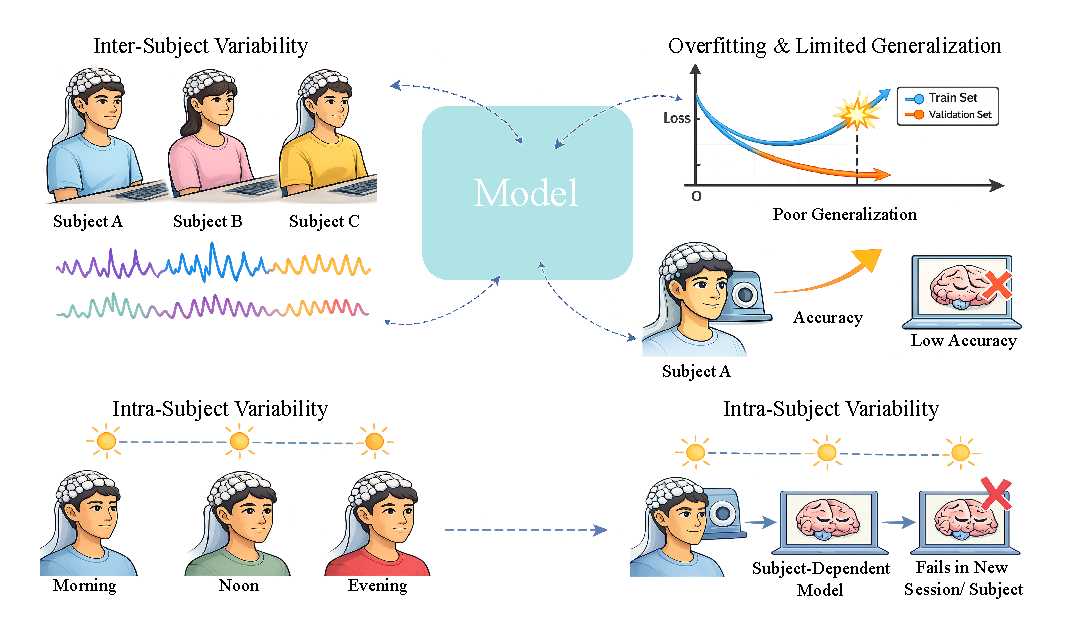
\includegraphics[width=\linewidth]{Figures/Problem 3.pdf}
    \caption{Inter- and intra-subject variability in \gls{eeg}-based \gls{bci} systems leading to overfitting and limited subject-independent generalization.}
    \label{fig:problem3}
\end{figure}

In addition to inter-subject differences, intra-subject variability introduces an additional challenge for robust \gls{eeg} modeling. \gls{eeg} signals recorded from the same individual may vary considerably across sessions due to fluctuations in attention, fatigue, emotional state, and subtle changes in acquisition conditions, resulting in nonstationary signal distributions over time~\cite{al2025emotion}. Such variability is particularly pronounced in real-world \gls{eeg}-based \glspl{bci} and in neurodevelopmental populations such as \gls{adhd}, where altered attentional control and increased behavioral variability have been shown to induce strong trial-to-trial and session-to-session fluctuations in neural activity~\cite{lenartowicz2018adhd}. This variability exacerbates the risk of overfitting, as learning algorithms may adapt to session-specific or noise-related patterns rather than stable neurophysiological features. Consequently, performance observed under optimistic or subject-dependent validation protocols often fails to generalize across sessions or recording conditions, reinforcing the vulnerability to domain shift and dataset-specific artifacts that has been consistently reported in subject-independent evaluations~\cite{wang2024dmmr}.

\subsection{Research Question}

\gls{eeg}-based \gls{bci} models face substantial constraints in their ability to generalize when exposed to distribution shifts across subjects, sessions, and recording conditions. These limitations are exacerbated by intrinsic properties of \gls{eeg} signals, including low spatial resolution induced by volume conduction effects, high susceptibility to noise and artifacts, and the nonlinear and nonstationary nature of brain dynamics. The interplay between signal degradation, heterogeneous neural patterns, and strong inter- and intra-subject variability undermines both the discriminative capability and the neurophysiological interpretability of existing learning models. Despite the adoption of deep learning, connectivity-based representations, and domain adaptation strategies, significant challenges remain in achieving robust, generalizable, and interpretable \gls{eeg} representations under real-world conditions.

This landscape motivates the research question: \textbf{How can an integrated and interpretable deep learning framework be designed for \gls{eeg}-based \gls{bci} systems to robustly model nonlinear and directed brain connectivity while improving generalization across subjects and sessions and mitigating the effects of noise and subject-specific variability?}